\section{Κατασκευή πλέγματος}

Όπως αναφέρθηκε και προηγουμένως, το πρόβλημα μοντελοποιείται ως αξονοσυμμετρικό επιλύεται σε διδιάστατο πλέγμα. Για την αυξηση της ακρίβειας των αριθμητικών μεθόδων, εφαρμόσθηκε πύκνωση στις περιοχές όπου έχουμε υψηλές κλίσεις και συγκεκριμένα, στην περιοχή γύρω απο τον δρομέα, στο τοίχωμα της αεροσύραγγας, και κοντά στον άξονα συμμετρίας όπου αναπτύσσεται ο ομόρρου της ανεμογεννήτριας. 

Η πύκνωση και η αραίωση του πλέγματος γίνεται με τη χρήση γεωμετρικής προόδου. Συμβολίζοντας με $p$ τη θέση ενός κόμβου, $dp$ την απόσταση μεταξύ δύο κόμβων, και $r$ τον λόγο της γεωμετρικής προόδου, η γεωμετρική πρόοδος περιγράφεται απο τις σχέσεις \ref{eq:geom}.
\begin{equation}
   \begin{gathered}
       \dfrac{dp_{k+1}}{dp_{k}} = r\\
       p_k = p_0 + dp_0\dfrac{r^k-1}{r-1}
   \end{gathered} 
    \label{eq:geom}
\end{equation}

\subsection{Κατασκευή πλέγματος κατά την ακτινική διεύθυνση}

Κατά την ακτινική διεύθυνση το πλέγμα χωρίστηκε σε τρείς περιοχές. Αρχικά στην περιοχή απο τον άξονα συμμετρίας έως την ακτίνα του δρομέα έχουμε ομοιόμορφο πλέγμα με μέγεθος {dy\_grid} που εισάγεται απο τον χρήστη. Έπειτα, το υπόλοιπο ακτινικό χωρίο χωρίζεται στα δύο. Απο τη θέση y=1 (ακτίνα δρομέα) έως το μέσο του υπολοιπόμενου χωρίου, έχουμε σταδιακή αραίωση με γεωμετρική πρόοδο. Ενώ απο το μέσο του χωρίου έως το τοίχωμα έχουμε σταδιακή πύκνωση με τον ίδιο λόγο γεωμετρικής προόδου, επομένως έχουμε αντικατωπτρισμό του πλέγματος που δημιουργήθηκε στην δεύτερη περιοχή. Το πλέγμα σε αυτές τις περιοχές ελέγχεται απο τον χρήστη εισάγωντας τον αριθμό των κελλιών σε κάθε περιοχή και τον λόγο της γεωμετρικής προόδου. Οι τρεις περιοχές και το παραγόμενο πλέγμα φαίνονται στο σχήμα \ref{fig:ygrid}.

Όπως φαίνεται και στο τμήμα του κώδικα \ref{lst:ycoarse}, με βάση τις εισόδους (αριθμός κελλιών) υπολογίζουμε μέσω της σχέσης \ref{eq:geom} το μήκος του πρώτου κελλιού στην πρόοδο (του μικρότερου), και χρησιμοποιώντας την ίδια σχέση υπολογίζουμε τη θέση του κάθε κόμβου.


\begin{figure}
    \begin{center}
        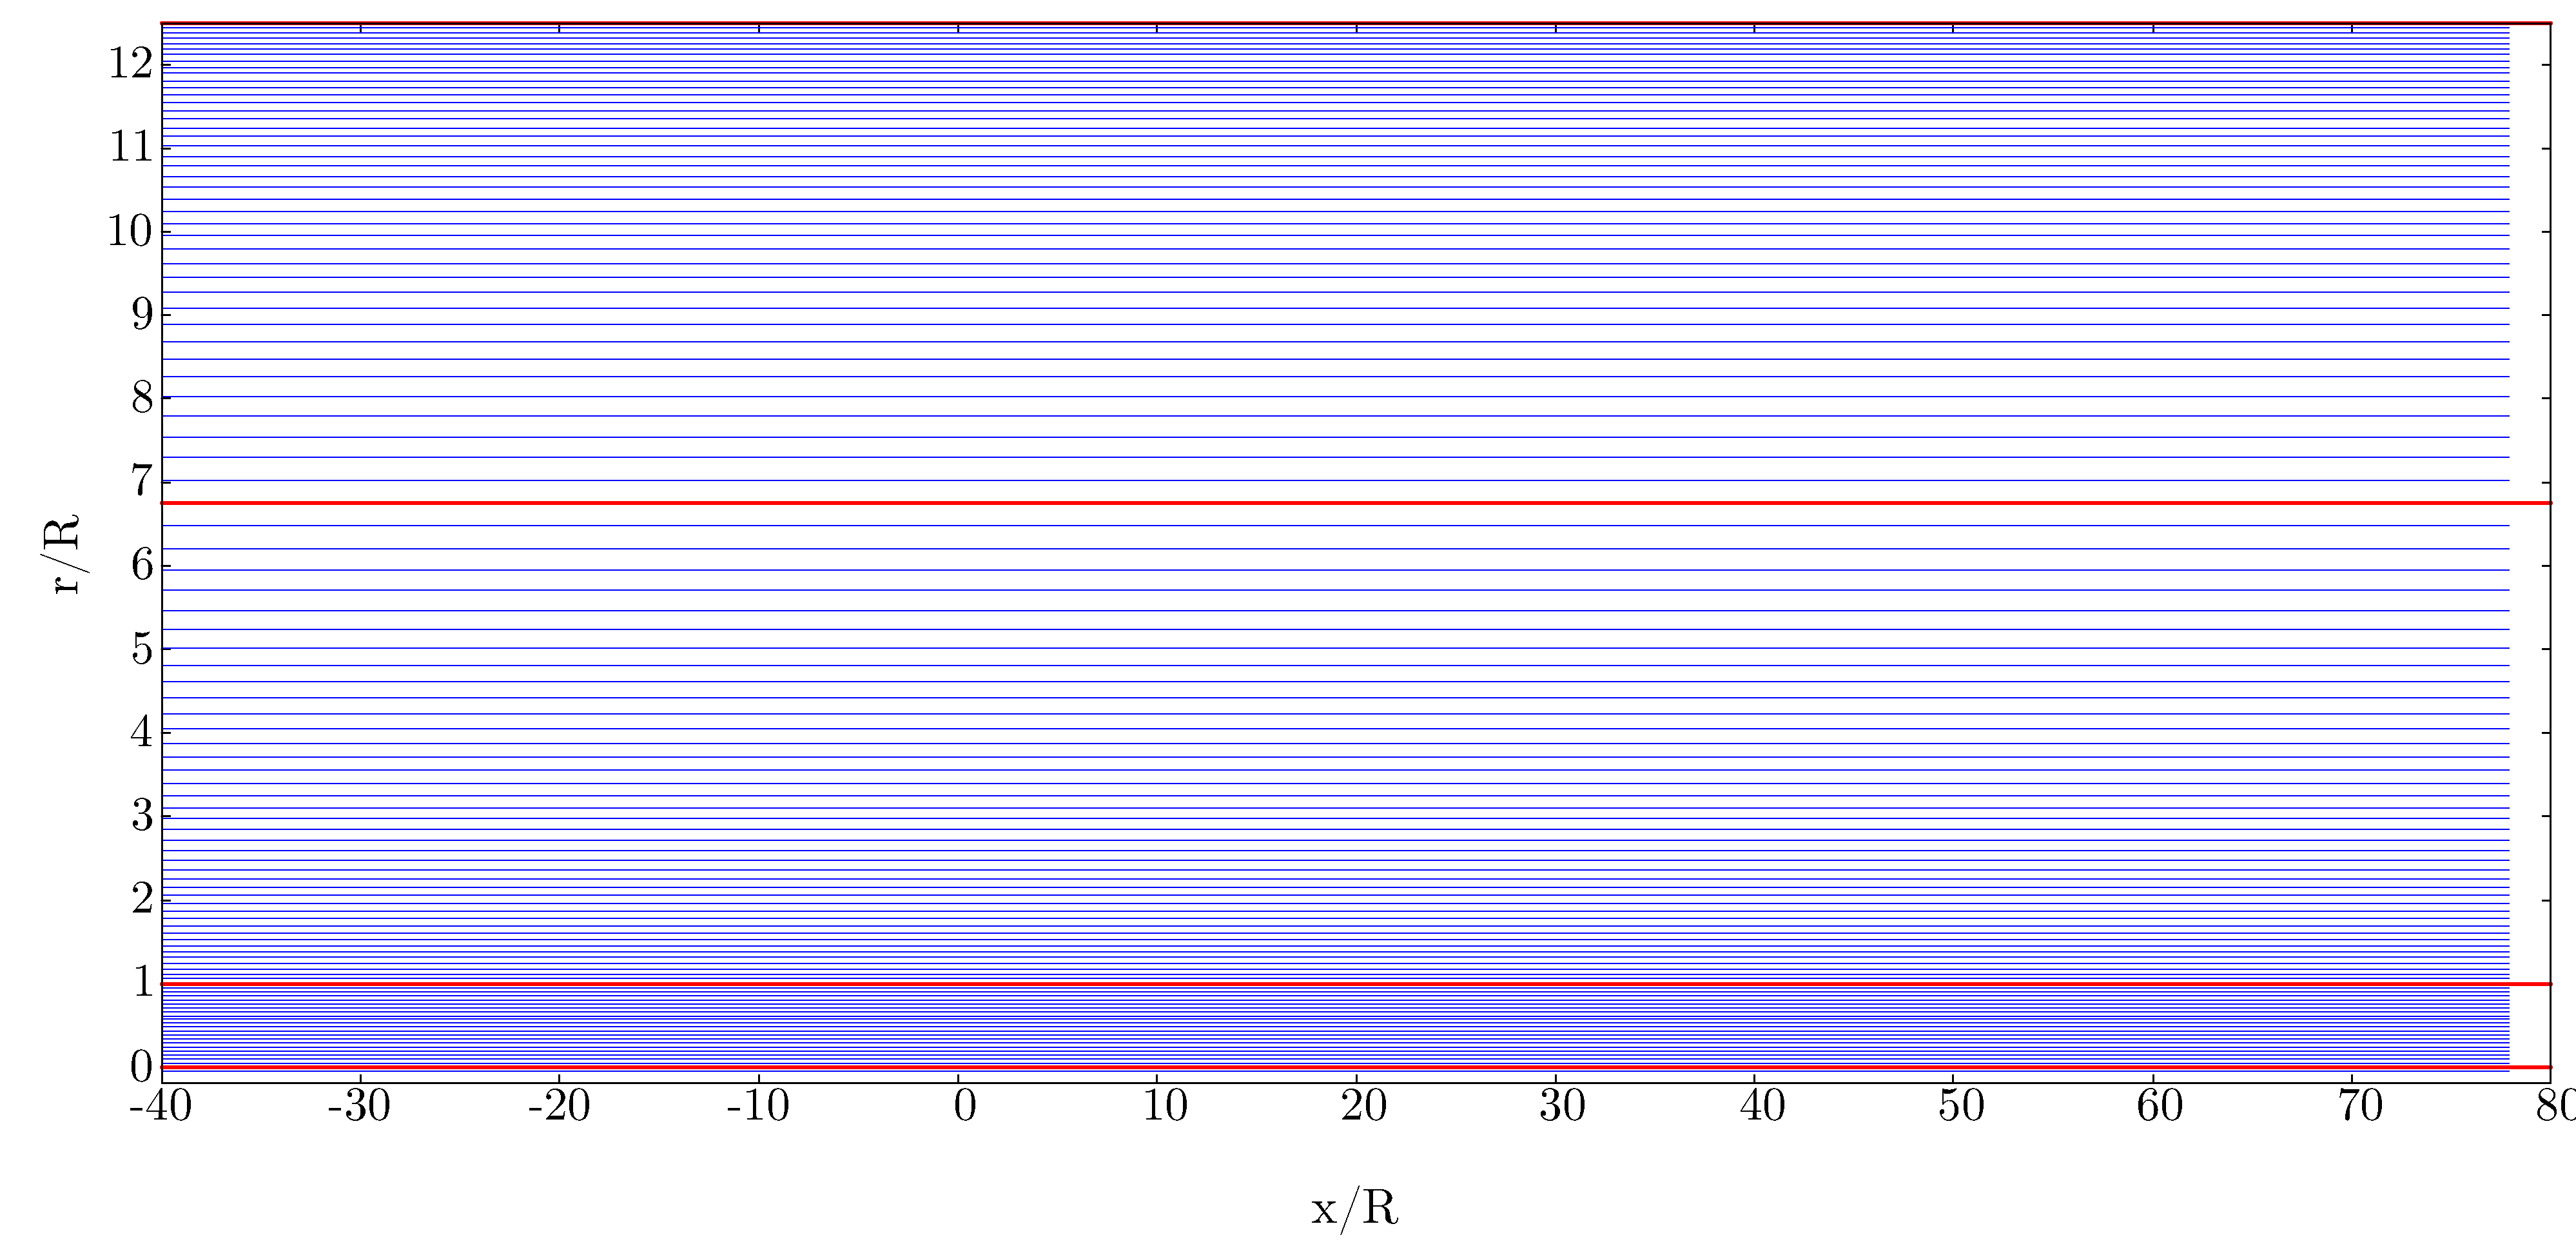
\includegraphics[width=0.95\textwidth]{figures/gridy.pdf}
    \end{center}
    \caption{Κόμβοι πλέγματος κατά την ακτινική διεύθυνση}
    \label{fig:ygrid}
\end{figure}


    \begin{lstlisting}[caption=\textrm{Κατασκευή ομοιόμορφου πλέγματος}, label={lst:yuni}, mathescape=true, breaklines=true, linewidth=.6\textwidth]
!--- Uniform grid in y-direction 
    !From y=ymin to y=1 (disk radius)

! Second point is on symmetry line
y_grid(2)=ymin 

do j=2,ngridy1-1
    y_grid(j+1)=y_grid(j) + dy_grid
enddo

! First point is symmetric to third
y_grid(1)=-y_grid(3) 
\end{lstlisting}

\begin{lstlisting}[caption=\textrm{Αραίωση πλέγματος}, label={lst:ycoarse}, mathescape=true, breaklines=true, linewidth=.6\textwidth]
!--- Non-uniform grid from ngridy1 to ngridy2
!--- From y=1 to y=y_mid 

! Calculate length of first cell in coarsening region
! using the number of cells
dy_grid_first= ((y_mid-1.d0) / (raty**(dble(ngridy2)) - 1.d0)) * (raty-1.d0)

do j=1,ngridy2
    y_grid(j+ngridy1)=y_grid(j+ngridy1-1) + dy_grid_first*raty**(j-1)
enddo
\end{lstlisting}

\begin{lstlisting}[caption=\textrm{Πύκνωση πλέγματος}, label={lst:yfine}, mathescape=true, breaklines=true, linewidth=.6\textwidth]
!--- Non-uniform grid from ngridy1 to ngridy2
!--- From y=y_mid to y=ymax 

do j=1,ngridy2
    ! Inverse raty to refine mesh
    y_grid(j+ngridy1+ngridy2)=y_grid(j+ngridy1+ngridy2-1) + dy_grid_first/raty**(j-1)*raty**(ngridy2-1)
enddo
\end{lstlisting}


\subsection{Κατασκευή πλέγματος κατά την αξονική διεύθυνση}

Όπως αναφέρθηκε και παραπάνω, στην αξονική διεύθυνση έχουμε ομοιόμορφο πλέγμα κοντά στον δρομέα, και σταδιακή αραίωση ανάντι και κατάντι αυτού. Ξανά, το μήκος των κελλιών στην ομοιόμορφη περιοχή ορίζεται απο τον χρήστη και είναι ίσο με το μήκος των κελλιών κατά την ακτινική διεύθυνση στο ομοιόμορφο τμήμα. Η κατανομή των κόμβων κατά την αξονική διεύθυνση φαίνεται στο σχήμα \ref{fig:gridx}.

\begin{figure}
    \begin{center}
        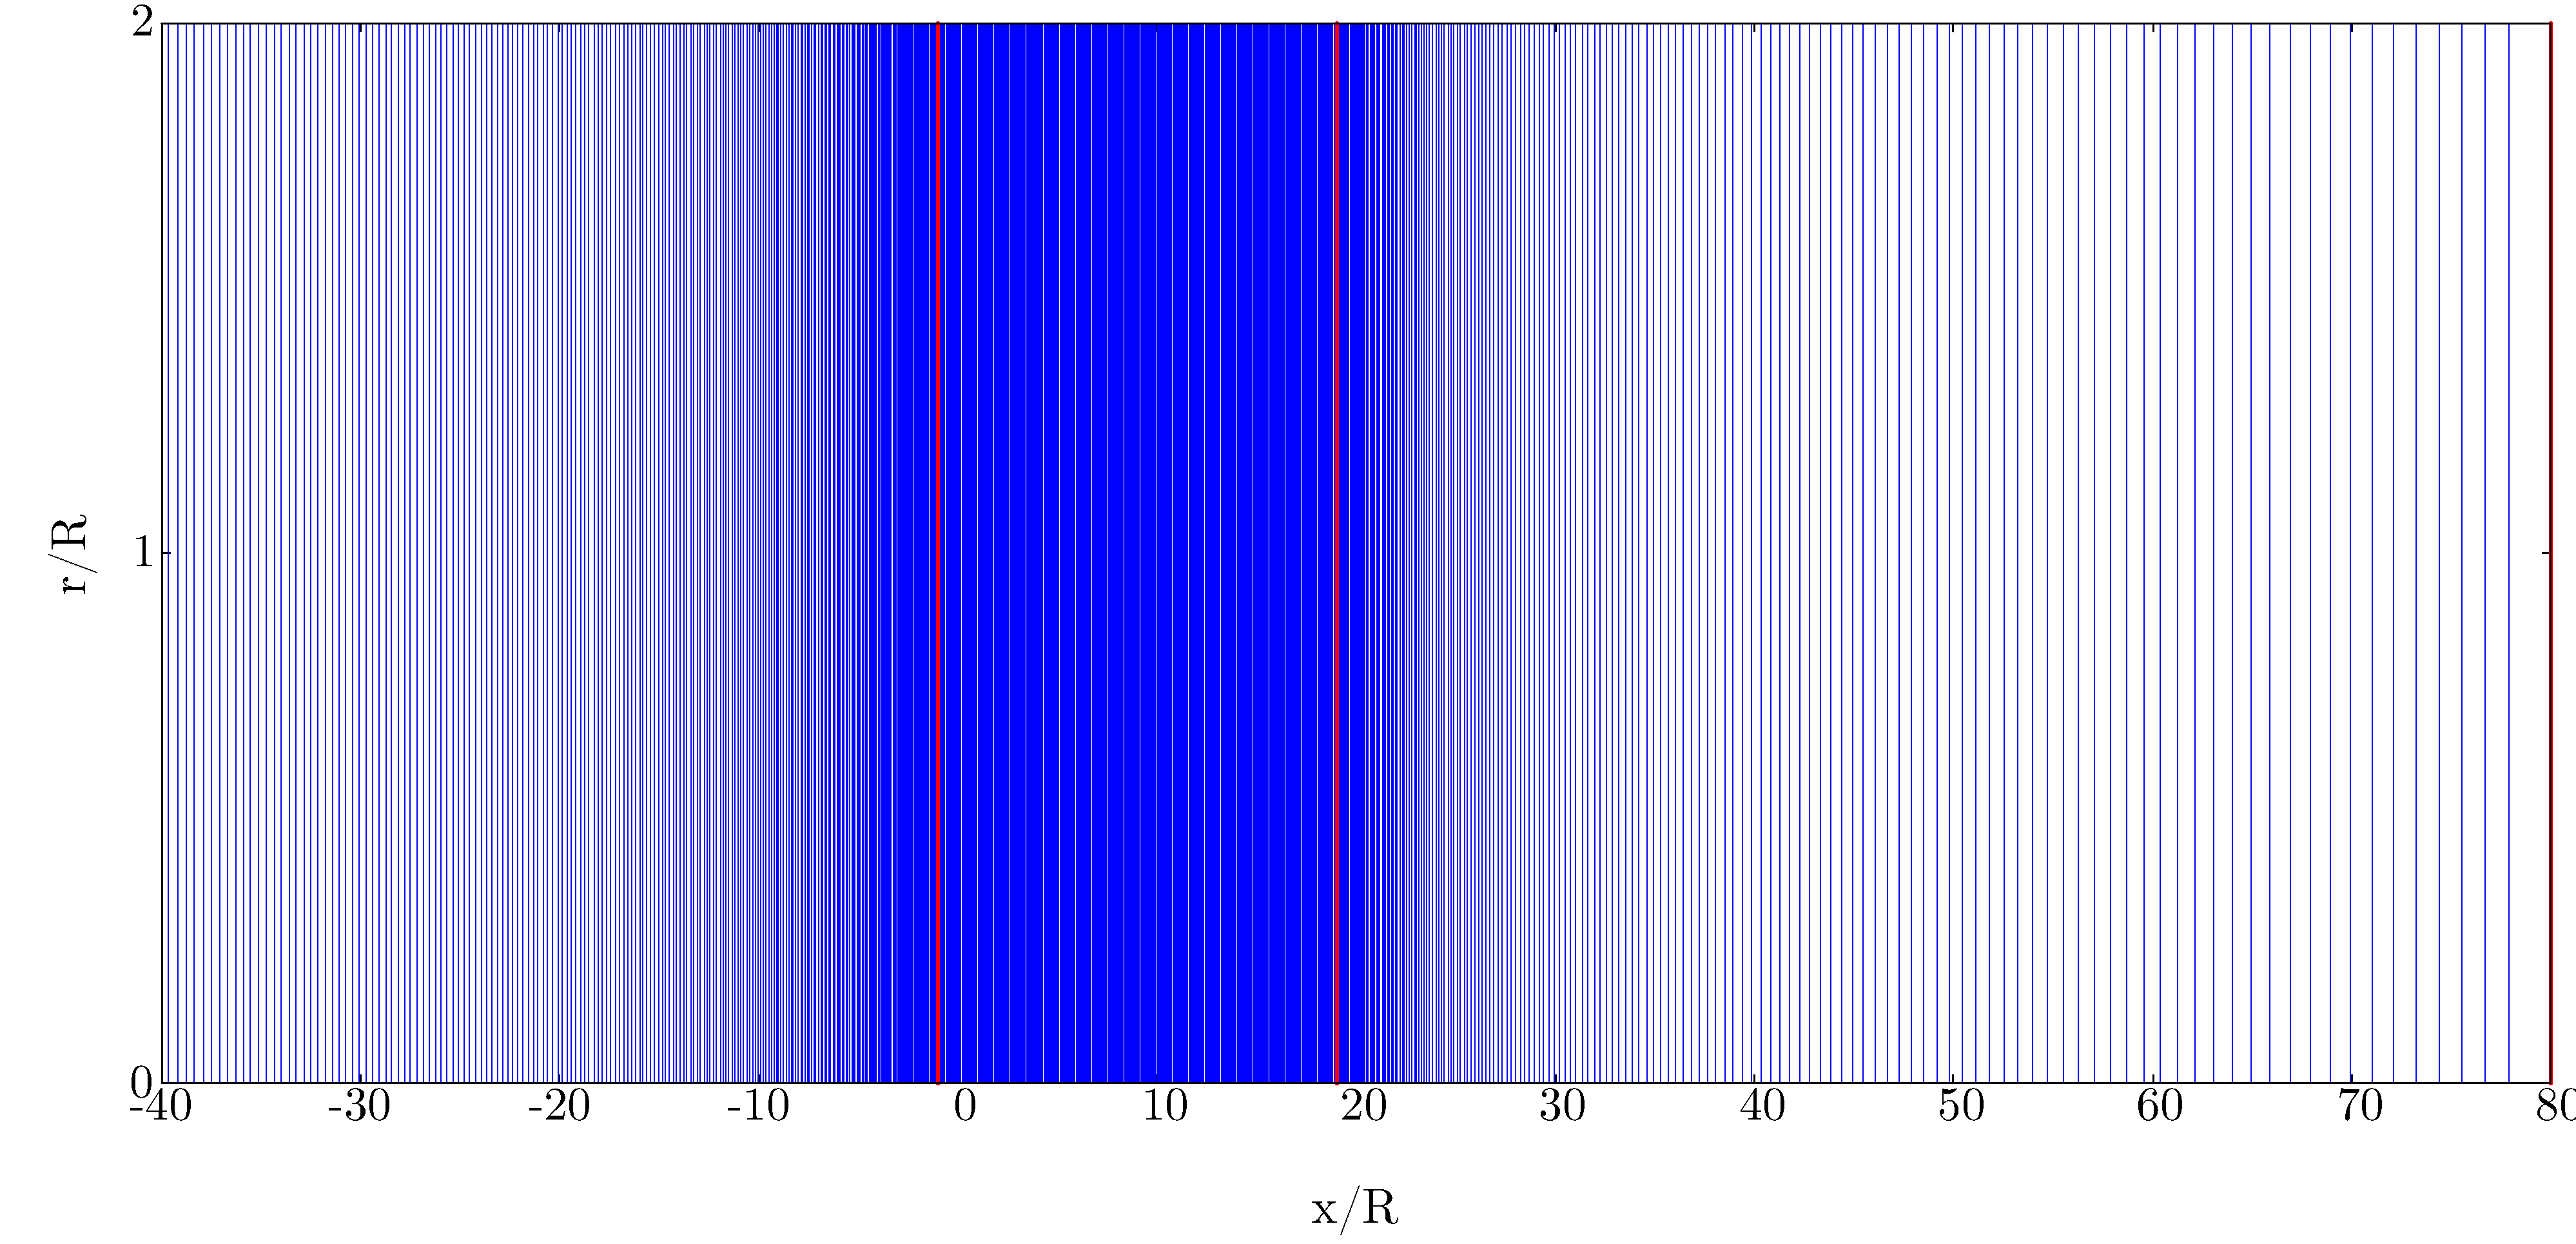
\includegraphics[width=0.95\textwidth]{figures/gridx.pdf}
    \end{center}
    \caption{Κόμβοι πλέγματος κατά την αξονική διεύθυνση}
    \label{fig:gridx}
\end{figure}

Παρακάτω φαίνονται τα τμήματα του κώδικα που δημιουργούν το πλέγμα για τις τρείς περιοχές κατά την αξονική διεύθυνση.

\begin{lstlisting}[caption=\textrm{Υπολογισμός παραμέτρων πλέγματος στην αξονική διεύθυνση}, label={lst:xgen}, mathescape=true, breaklines=true, linewidth=.6\textwidth]
!-- x-grid 
write(*,*) "Target Uni Dx=", dx_uni_tar
! Correct uniform spacing to intersect x=-1 and x=0
dx_uni_cor = 10**(LOG10(1.d0)-LOG10(dble(ceiling(10**(LOG10(1.d0)-LOG10(dx_uni_tar))))))
! Calculate number of grid points
ngridx2 = ceiling(xuni / dx_uni_cor)
dx_grid2 = dx_uni_cor
dx_grid1 = dx_uni_cor 
write(*,*) 'dx_grid1=', dx_grid1

ngridx1 = int(dlog(1.d0+xmin*(1.d0-ratx1)/dx_grid1)/dlog(ratx1))

ngridx3 = int(dlog(1.d0-(xmax-xuni)*(1.d0-ratx2)/dx_grid1)/dlog(ratx2))

ngridx=ngridx1+ngridx2+ngridx3
! Save the index of rotor axial position
x0ind = ngridx1+ngridx2/xuni
\end{lstlisting}

\begin{lstlisting}[caption=\textrm{Αραίωση πλέγματος ανάντι δρομέα}, label={lst:xup}, mathescape=true, breaklines=true, linewidth=.6\textwidth]
! Upstream coarsening (x < -1) with ratx1 ratio
x_grid(ngridx1)=-1.d0
do i=1,ngridx1-1
    x_grid(ngridx1-i)=x_grid(ngridx1-i+1)-dx_grid1*ratx1**(i-1)
enddo
\end{lstlisting}

\begin{lstlisting}[caption=\textrm{Ομοιόμορφο πλέγμα κοντά στον δρομέα}, label={lst:xuni}, mathescape=true, breaklines=true, linewidth=.6\textwidth]
    ! Uniform grid -1 < x < XUNI-1
    do i=1,ngridx2
        x_grid(ngridx1+i)=x_grid(ngridx1+i-1)+dx_grid2
    enddo
\end{lstlisting}

\begin{lstlisting}[caption=\textrm{Αραίωση πλέγματος κατάντι δρομέα}, label={lst:xdown}, mathescape=true, breaklines=true, linewidth=.6\textwidth]
! Downstream coarsening (x > XUNI-1) with ratx2 ratio 
do i=1,ngridx3
    x_grid(ngridx1+ngridx2+i)=x_grid(ngridx1+ngridx2+i-1)+dx_grid2*ratx2**(i-1)
enddo
\end{lstlisting}
Όπως φαίνεται και στο τμήμα του κώδικα \ref{lst:xgen}, το πλήθος των κόμβων για τα δύο τμήματα που αραιώνουμε, υπολογίζεται ώστε προσεγγιστικά να φτάνει το πλέγμα έως τα όρια που έχει ορίσει ο χρήστης. Θα μπορούσαμε εναλλακτικά να εισάγουμε το πλήθος των κόμβων και να λύσουμε την εξίσωση \ref{eq:geom} ωστε να καθορίσουμε το απαιτούμενο μήκος του πρώτου κελλιού. Ωστόσο, δεν μας ενδιαφέρει να πετύχουμε ακριβώς τη θέση εισόδου και εξόδου που ορίζει ο χρήστης, αφού απλά ενδιαφερόμαστε να έχουμε ικανοποιητικό μήκος ώστε να μπορούμε να εφαρμόσουμε συνοριακές συνθήκες που δεν θα επηρεάζονται απο τις συνθήκες κοντά στον δρομέα, δηλαδή να έχουμε αποκατεστημένη ροή.

Έτσι, σε αυτή την περίπτωση, είναι προτιμότερο να έχουμε ομαλή μετάβαση απο το τμήμα ομοιόμορφου πλέγματος στα τμήματα της αράιωσης διατηρώντας ίδιο μήκος κελλιού στο σύνορο των περιοχών.

\subsection{Παράμετροι \& εικόνες πλέγματος}

Οι τελικές γεωμετρικές παράμετροι και οι παράμετροι που αφορούν το πλέγμα και αναφέρθηκαν παραπάνω παρατίθενται στον πίνακα \ref{tab:geom_mesh}.


\begin{table}[h!]
    \begin{center}
        \begin{tabular}[c]{|r|c|l|}
            \hline
            XMIN & -40 & Αρχή υπολογιστικού χωρίου\\
            XMAX & 80 & Τέλος υπολογιστικού χωρίου\\
            XUNI & 20 & Μήκος τμήματος ομοιόμορφου πλέγματος\\
            YMIN & 0  & Ελάχιστη ακτινική θέση\\
            YMAX & 12.5 & Μέγιστη ακτινική θέση\\
            NGRIDX1 & 91 & Πλήθος κόμβων αραίωσης - αξονικά\\
            NGRIDX & 582 & Συνολικό πλήθος κόμβων - αξονικά\\
            NGRIDY1 & 41 & Πλήθος κόμβων αραίωσης - ακτινικά\\
            NGRIDY & 102 & Συνολικό πλήθος κόμβων - ακτινικά\\
            dx\_uni & 0.05 & Μέγεθος κελλιού - ομοιόμορφο πλέγμα\\
            RATX1 & 1.01 & Λόγος ΓΠ ανάντι\\
            RATX2 & 1.02 & Λόγος ΓΠ κατάντι\\
            RATY & 1.04 & Λόγος ακτινικής πύκνωσης\\
            \hline
        \end{tabular}
    \end{center}
    \caption{Τελικές γεωμετρικές παράμετροι και παράμετροι πλέγματος}
    \label{tab:geom_mesh}
\end{table}

Στα ακόλουθα διαγράμματα παρουσιάζεται η τελική μορφή του πλέγματος σε ολόκληρο το χωρίο και εστιασμένο στις περιοχές ενδιαφέροντος. Η θέση του δρομέα σημειώνεται με κόκκινη συμπαγή γραμμή.

\begin{figure}[h!]
    \begin{center}
        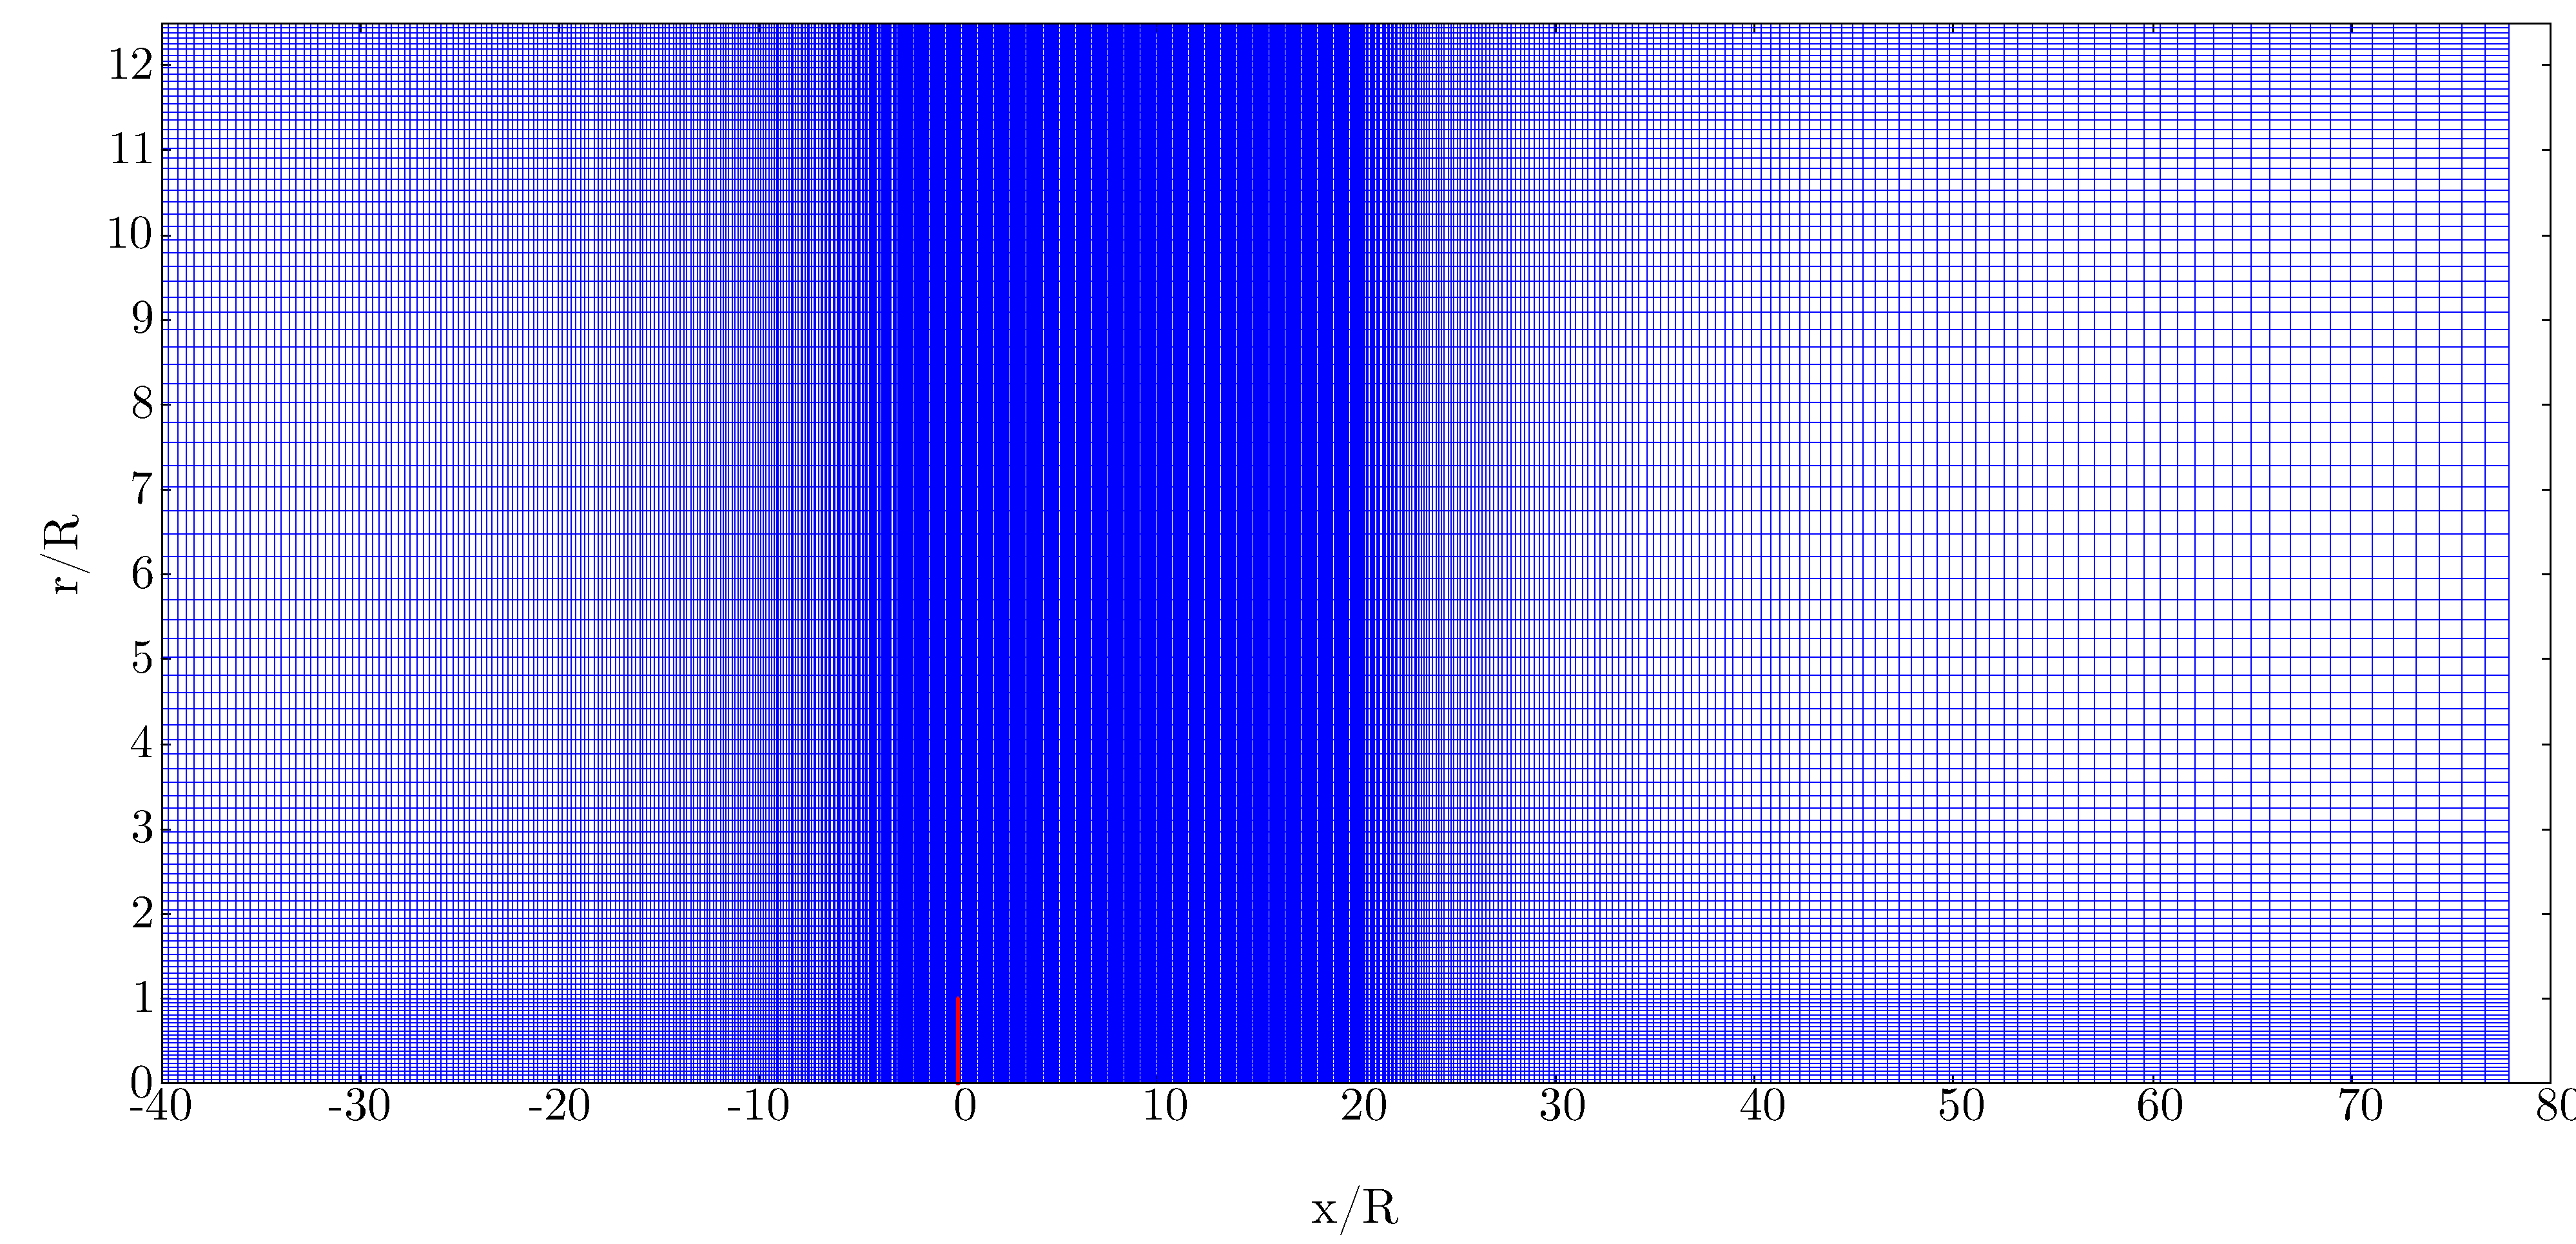
\includegraphics[width=0.95\textwidth]{figures/meshAll.pdf}
    \end{center}
    \caption{Συνολική εικόνα πλέγματος}
    \label{fig:meshAll}
\end{figure}

\begin{figure}[h!]
    \begin{center}
        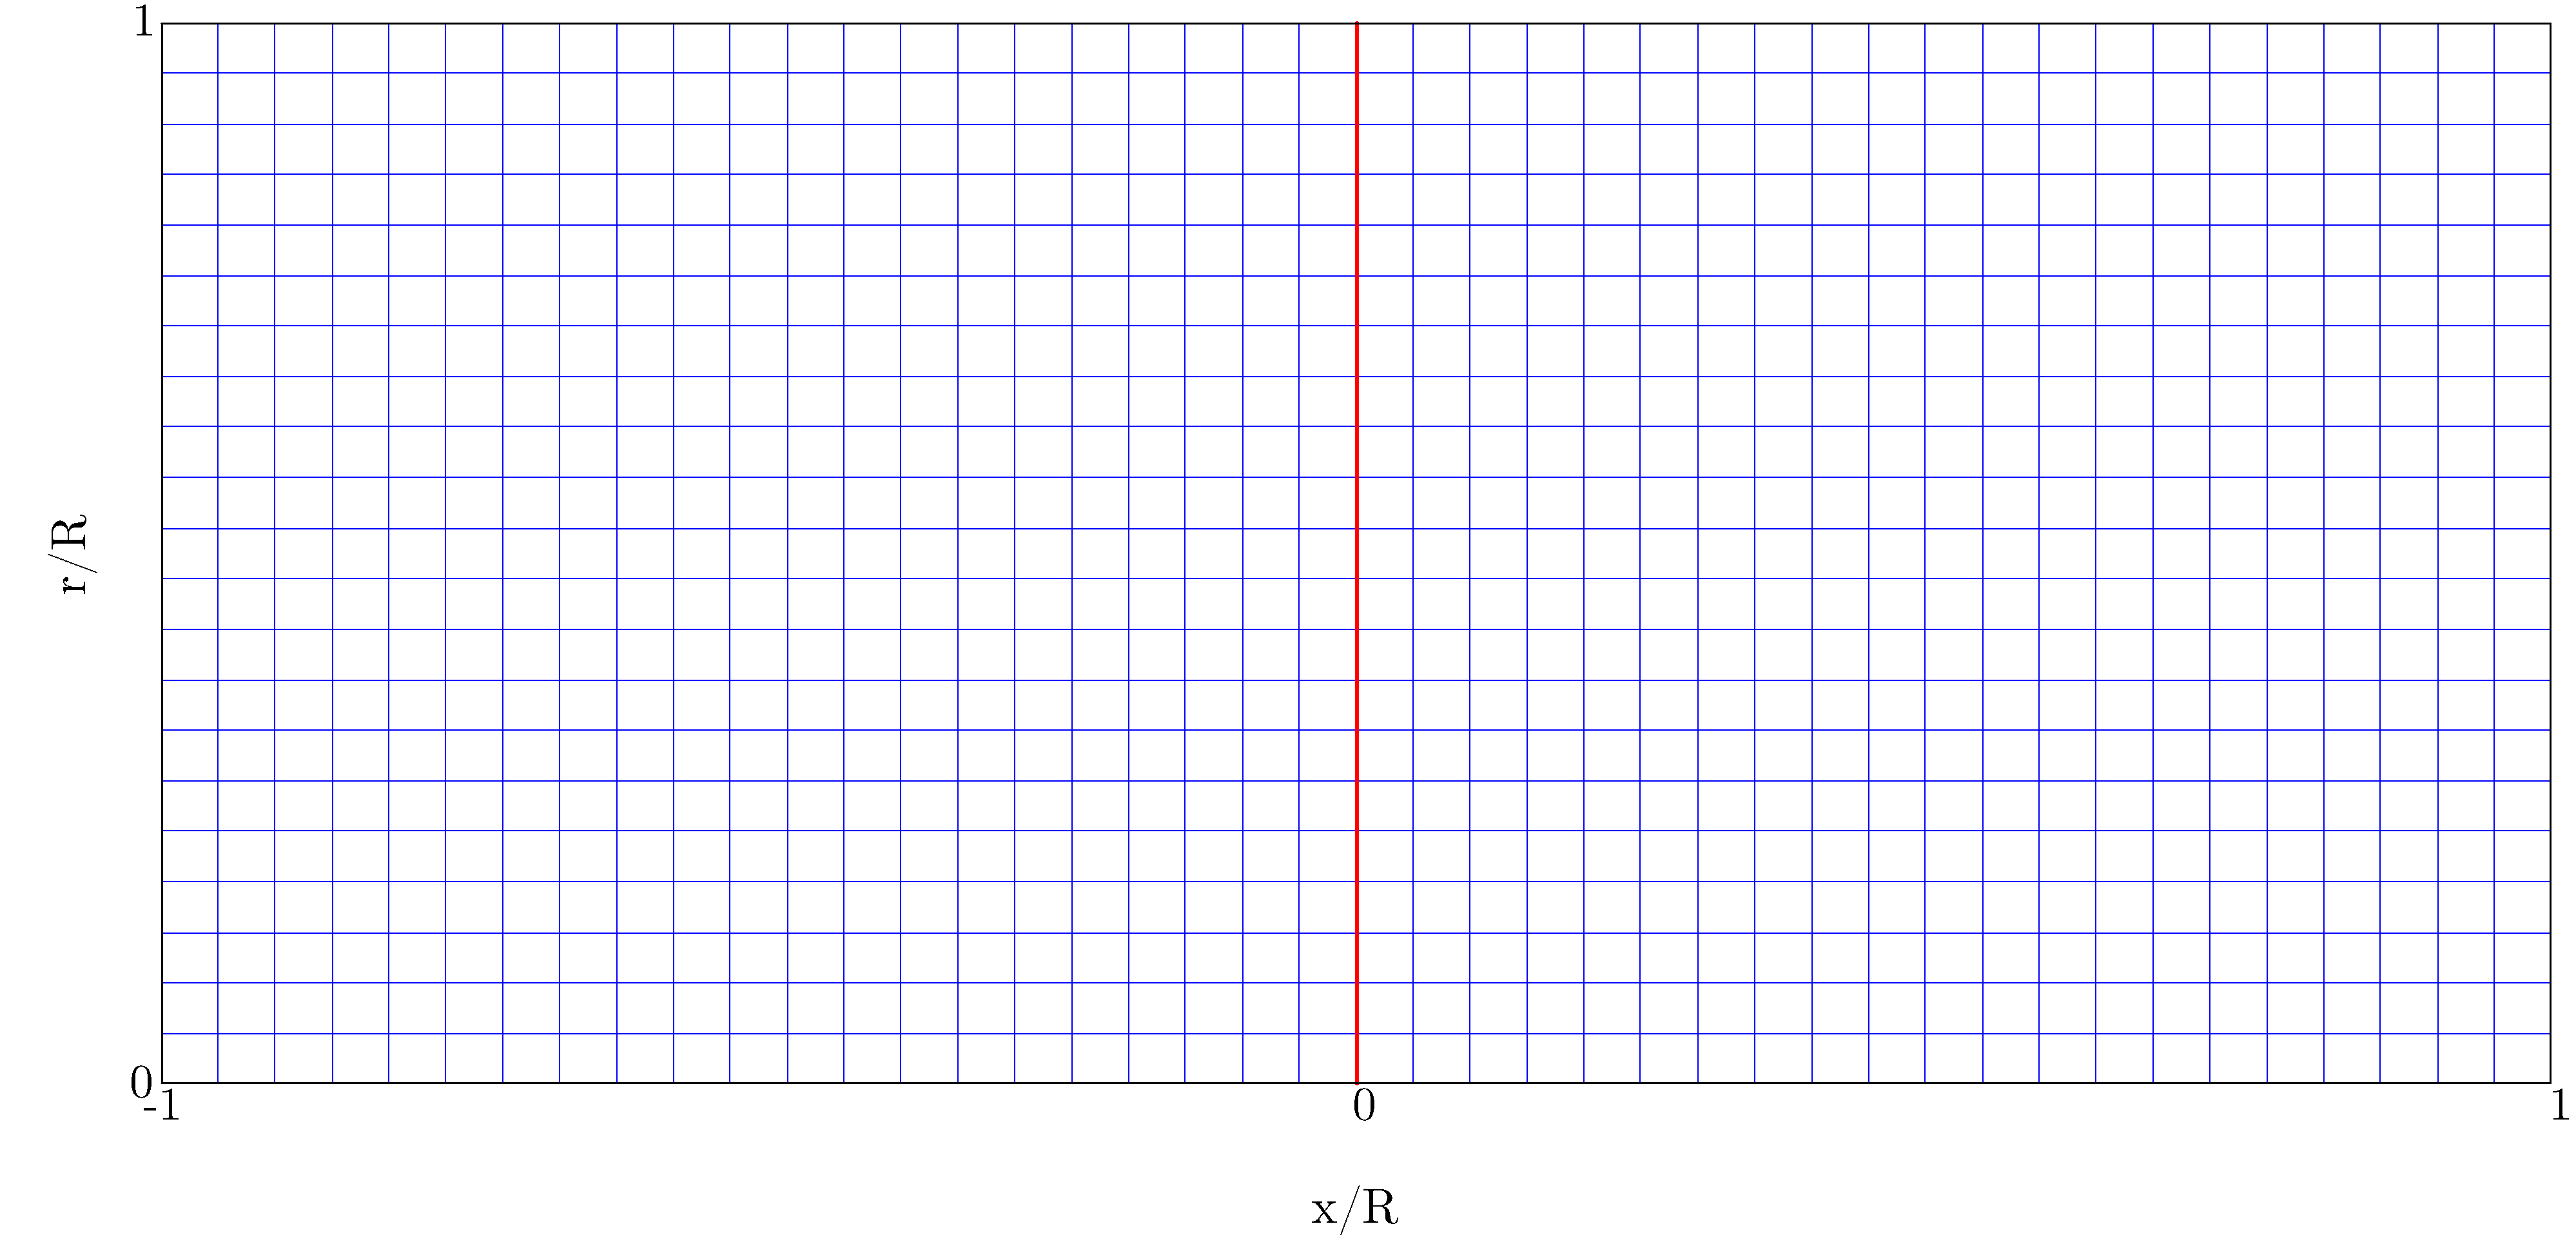
\includegraphics[width=0.95\textwidth]{figures/meshRotor.pdf}
    \end{center}
    \caption{Περιοχή δρομέα - ομοιόμορφο πλέγμα}
    \label{fig:meshRotor}
\end{figure}

\begin{figure}[h!]
    \begin{center}
        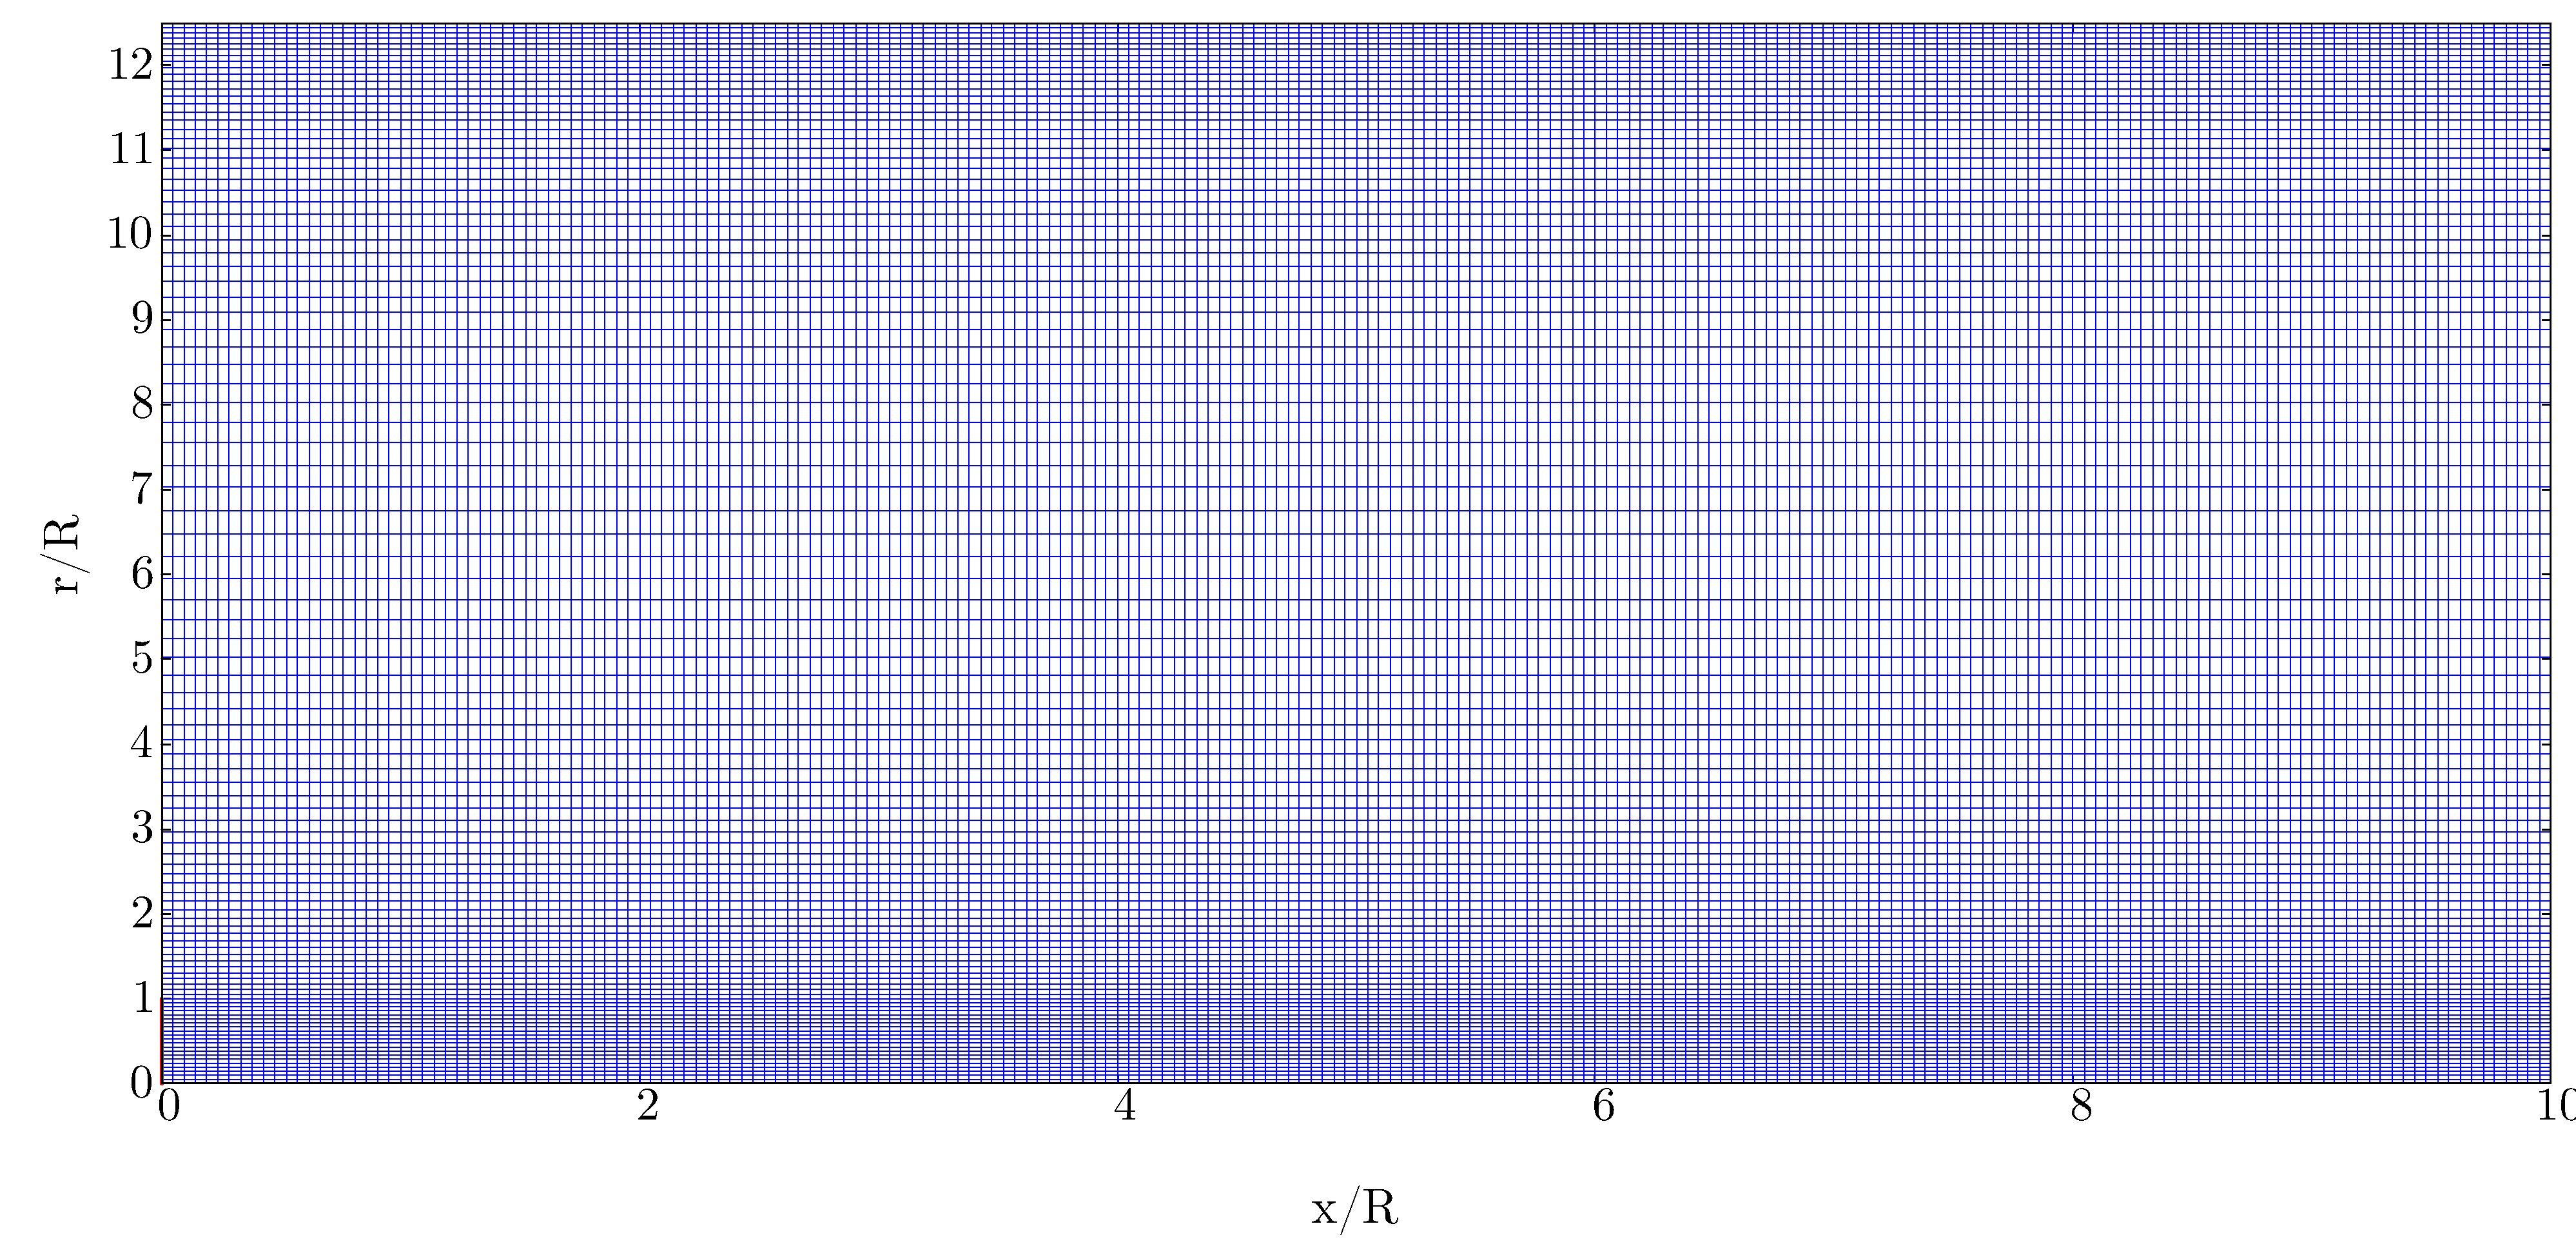
\includegraphics[width=0.95\textwidth]{figures/meshDown.pdf}
    \end{center}
    \caption{Περιοχή κατάντι δρομέα}
    \label{fig:meshDown}
\end{figure}
